%% This section analyze results of the benchmark and highlights the most interesting findings. %% are presented in Section~\ref{sec:}.
Figures\,\ref{fig:socapps_plots} and~\ref{fig:cfdapps_plots} summarize major benchmarking results
for social science and CFD applications respectively.
For each application, we include two plots:
the first one -- scalability plot -- illustrates the change
in the total ellapsed time with the grows of the number of MPI processes for all testbeds,
whereas the second one -- metrics plot -- present all metrics measured for Intel Xeon Gold 6140 with different number of MPI processes.
Intel Xeon Gold 6140 has been  chosen to report details on measured metrics 
since it demonstrated the best performance compared to other testbeds (see Section\,\ref{sec:summary}).
Reports \cite{2017:coegss_benchmark1,2018:coegss_benchmark2} contain the same information
for other testbeds besides Intel Xeon Gold 6140.
Both figures\,\ref{fig:socapps_plots} and~\ref{fig:cfdapps_plots} share identical legends.
Note that scalability plot for HWRF application (Figure\,\ref{fig:hwrf_scalability}) lacks information about ARM Hi1616 and IBM Power8+.
We failed to port HWRF on those architectures.

%% 1 row - IPF
\begin{figure}[t]
  \centering
  \begin{subfigure}[t]{0.48\textwidth}
    \centering
    \begin{tikzpicture}[scale=1, baseline]
      \begin{customlegend}[legend columns=1,legend style={font=\tiny, column sep=2ex},
          legend entries={Eagle/Intel\ Xeon\ E5-2697 v3,
            ARM Hi1616,
            Intel\ Xeon\ Gold 6140,
            AMD Epyc 7551,
            Power8+ S822LC
        }]
        \addlegendimage{mark=otimes,solid}
        \addlegendimage{mark=square,solid}
        \addlegendimage{mark=*,solid}
        \addlegendimage{mark=star,solid}
        \addlegendimage{mark=|,solid}
      \end{customlegend}
    \end{tikzpicture}
  \end{subfigure}\hfill
  \begin{subfigure}[t]{0.48\textwidth}
    \centering
    \begin{tikzpicture}[scale=1, baseline]
      \begin{customlegend}[legend columns=1,legend style={font=\tiny, column sep=2ex},
          legend entries={Execution time ,
            Memory use,
            No. of system file inputs,
            No. of system file outputs
        }]
        \addlegendimage{mark=*,solid}
        \addlegendimage{mark=square,solid}
        \addlegendimage{mark=star,solid}
        \addlegendimage{mark=otimes,solid}
      \end{customlegend}
    \end{tikzpicture}
  \end{subfigure}\bigbreak

  \begin{subfigure}[t]{0.48\textwidth}
    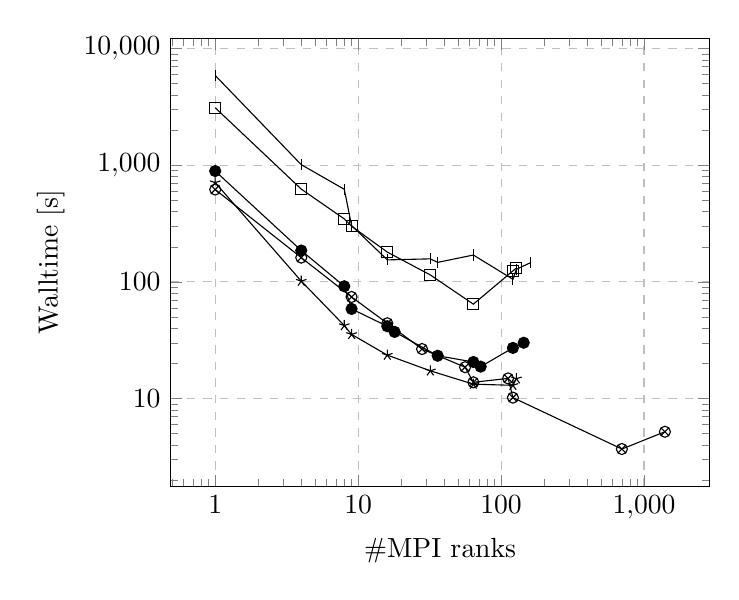
\begin{tikzpicture}[scale=1, baseline]
      \begin{axis}[
          xmode=log,
          ymode=log,
          log ticks with fixed point,
          scaled y ticks=real:1e3
          axis lines = left,
          xlabel = \#MPI ranks,
          ylabel = {Walltime [s]},
          legend style={at={(0.5,-0.2)},
            anchor=north,legend columns=1},
          xmajorgrids=true,
          ymajorgrids=true,
          grid style=dashed,
        ]
        %ARM
        \addplot [
          domain=1:150, 
          color=black,
          mark=square,
        ]
        coordinates {                 (1,3107.3)(4,624.3)(8,346.5)(9,299.7)(16,180.1)(32,114.7)(64,64.5)(121,124.3)(128,131.5)};
        %                \addlegendentry{ARM Hi1616}
        %Intel 6140
        \addplot [
          domain=1:150, 
          color=black,
          mark=*,
        ]
        coordinates {                   (1,891.2)(4,185.8)(8,91.8)(9,58.7)(16,41.7)(18,37.3)(36,23.3)(64,20.6)(72,18.8)(121,27.2)(144,30.1)};
        %                \addlegendentry{Intel\ Xeon\ Gold 6140}
        %AMD Epyc
        \addplot [
          domain=1:150, 
          color=black,
          mark=star,
        ]
        coordinates {
          (1,709.9)(4,101.6)(8,42.3)(9,35.5)(16,23.6)(32,17.3)(64,13.3)(121,13.0)(128,14.8)};
        %               \addlegendentry{AMD Epyc 7551}
        %Eagle
        \addplot [
          domain=1:1400, 
          color=black,
          mark=otimes,
        ]
        coordinates {                    (1,618.9)(4,161.5)(9,74.3)(16,44.2)(28,26.6)(56,18.6)(64,13.8)(112,14.9)(121,10.2)(700,3.7)(1400,5.2)
        };
        %               \addlegendentry{Eagle/Intel\ Xeon\ E5-2697 v3}
        %Power
        \addplot [
          domain=1:150, 
          color=black,
          mark=|,
        ]
        coordinates {
          (1,5878.0)(4,1010.5)(8,621.8)(9,304.1)(16,154.4)(32,157.6)(36,147)(64,170)(121,105.3)(128,128.3)(160,145.8)
        };
        %                \addlegendentry{Power8+ S822LC}
      \end{axis}
    \end{tikzpicture}
    \caption{IPF scalability}
    \label{fig:ipf_scalability}
  \end{subfigure}\hfill
  \begin{subfigure}[t]{0.48\textwidth}
    \centering
    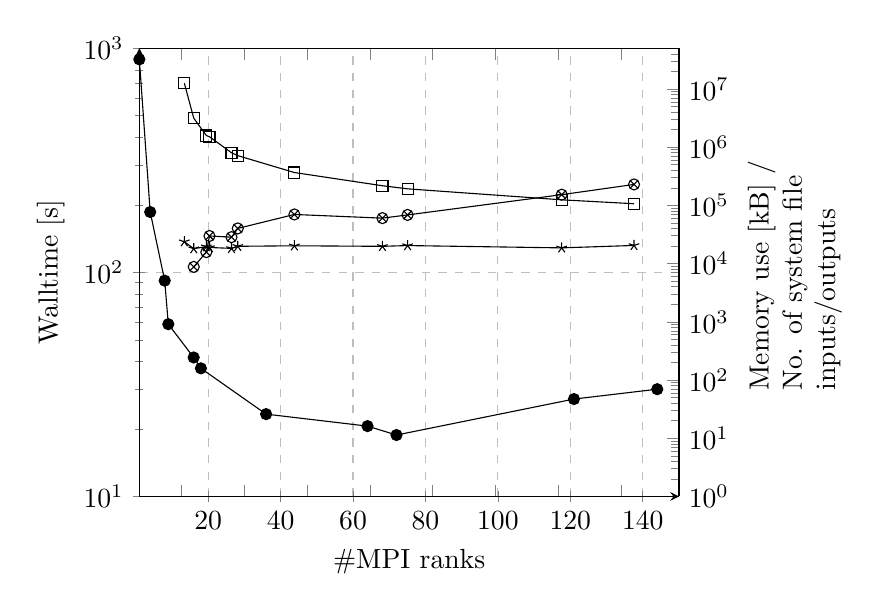
\begin{tikzpicture}[scale=1, baseline]
      \begin{axis}[
          %    width=1\textwidth,
          axis y line*=left,
          axis lines = left,
          xlabel = \#MPI ranks,
          ylabel = {Walltime [s]},
          xmajorgrids=true,
          ymajorgrids=true,
          grid style=dashed,
          xmin=1, xmax=150,
          ymode=log,
          ymin=10, ymax=1000,
        ]
        %Execution time
        \addplot [
          domain=1:70, 
          color=black,
          mark=*,
        ]
        coordinates {                   (1,891.2)(4,185.8)(8,91.8)(9,58.7)(16,41.7)(18,37.3)(36,23.3)(64,20.6)(72,18.8)(121,27.2)(144,30.1)};
        \label{ipf_execution_time}
      \end{axis}
      \begin{axis}[
          %                xmode=log,
          ymode=log,
          xticklabel=\empty,
          axis y line*=right,
          scaled ticks=false,
          y tick label style={/pgf/number format/.cd,sci,sci e},
          ymin=1, ymax=50000000,
          ylabel style={text width=3cm},
          ylabel = {Memory use {[kB]} {/} No. of system file inputs/outputs},
          legend style={at={(0.5,-0.2)},
            anchor=north,legend columns=1},
          grid style=dashed,
        ]
        \addlegendimage{/pgfplots/refstyle=ipf_execution_time}
        %                \addlegendentry{Execution time}
        %RAM
        \addplot [
          domain=1:70, 
          color=black,
          mark=square,
        ]
        coordinates {(1,12510916)(4,3140960)(8,1579868)(9,1505996)(16,800212)(18,713344)(36,365920)(64,216960)(72,191912)(121,124292)(144,106468)};
        %                \addlegendentry{Memory use}
        %#inputs
        \addplot [
          domain=1:70, 
          color=black,
          mark=star,
        ]
        coordinates {(1,23752)(4,18024)(8,19488)(9,18888)(16,18224)(18,19792)(36,20192)(64,19768)(72,20368)(121,18592)(144,20464)};
        %              \addlegendentry{No. of system file inputs}
        %#outputs
        \addplot [
          color=black,
          mark=otimes,
        ]
        coordinates {(1,0)(4,8760)(8,15728)(9,29744)(16,28400)(18,40128)(36,69664)(64,60248)(72,68416)(121,152384)(144,228360)};
        %                   \addlegendentry{No. of system file outputs}
      \end{axis}
    \end{tikzpicture}
    \caption{IPF on Intel\ Xeon\ Gold 6140}
    \label{fig:ipf_intel_gold}
  \end{subfigure}\bigbreak
  %      \caption{Results for IPF}
  %\end{figure}

  %% 3 row - \textsf{ABM4Py}
  %\begin{figure}[ht]
  %\centering
  \begin{subfigure}[t]{0.48\textwidth}
    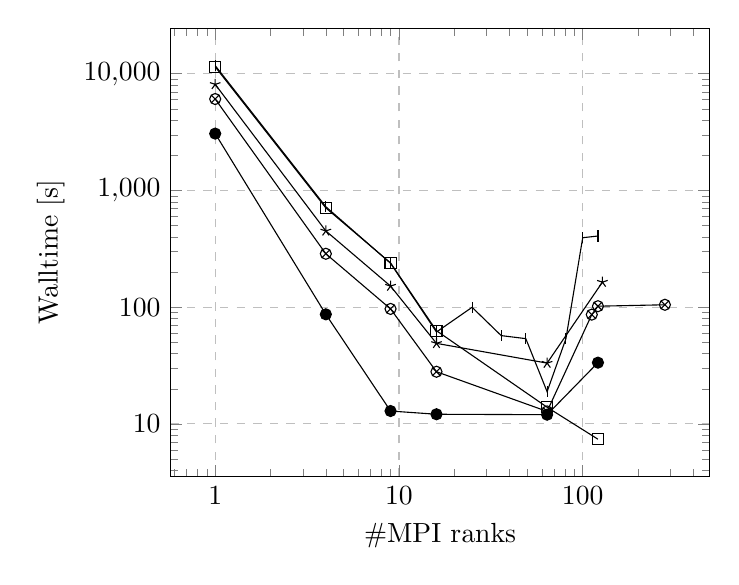
\begin{tikzpicture}[scale=1, baseline]
      \begin{axis}[
          xmode=log,
          ymode=log,
          log ticks with fixed point,
          scaled y ticks=real:1e3
          axis lines = left,
          xlabel = \#MPI ranks,
          ylabel = {Walltime [s]},
          %            legend style={at={(0.5,-0.2)},
          %            	    anchor=north,legend columns=1},
          xmajorgrids=true,
          ymajorgrids=true,
          grid style=dashed,
        ]
        %ARM
        \addplot [
          domain=1:150, 
          color=black,
          mark=square,
        ]
        coordinates {                 (1,11463.3)(4,708.9)(9,239.5)(16,62.9)(64,13.9)(121,7.4)};
        %                \addlegendentry{ARM Hi1616}
        %Intel 6140
        \addplot [
          domain=1:150, 
          color=black,
          mark=*,
        ]
        coordinates {                   (1,3071.5)(4,86.9)(9,12.9)(16,12.1)(64,12.0)(121,33.5)};
        %                \addlegendentry{Intel\ Xeon\ Gold 6140}
        %AMD Epyc
        \addplot [
          domain=1:150, 
          color=black,
          mark=star,
        ]
        coordinates {
          (1,8114.8)(4,450.3)(9,151.7)(16,49.0)(64,33.2)(128,164)};
        %                \addlegendentry{AMD Epyc 7551}
        %Eagle
        \addplot [
          domain=1:1400, 
          color=black,
          mark=otimes,
        ]
        coordinates {                    (1,6077.3)(4,287)(9,96.7)(16,28)(64,12.8)(112,86.4)(121,102)(280,104.9)
        };
        %                \addlegendentry{Eagle/Intel\ Xeon\ E5-2697 v3}
        %Power
        \addplot [
          domain=1:150, 
          color=black,
          mark=|,
        ]
        coordinates {
          (1,11751.7)(4,725.9)(9,237.9)(16,61.3)(25,99.8)(36,57.1)(49,53.8)(64,18.9)(81,53.7)(100,394.1)(121,407.3)
        };
        %                \addlegendentry{Power8+ S822LC}
      \end{axis}
    \end{tikzpicture}
    \caption{\textsf{ABM4Py}/GG scalability}
    \label{fig:abms_scalability}
  \end{subfigure}\hfill
  \begin{subfigure}[t]{0.48\textwidth}
    \centering
    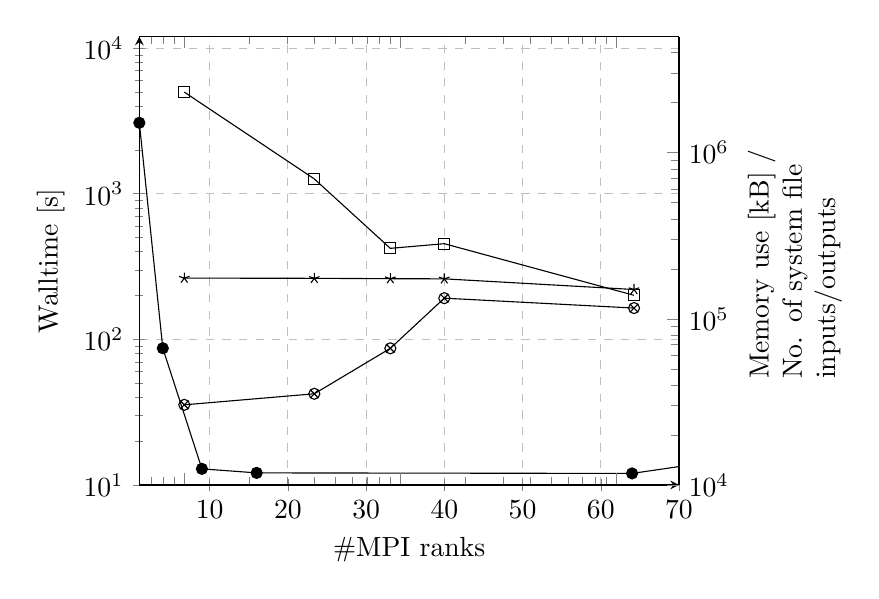
\begin{tikzpicture}[scale=1, baseline]
      \begin{axis}[
          %    width=1\textwidth,
          axis y line*=left,
          axis lines = left,
          xlabel = \#MPI ranks,
          ylabel = {Walltime [s]},
          xmajorgrids=true,
          ymajorgrids=true,
          grid style=dashed,
          xmin=1, xmax=70,
          ymode=log,
          ymin=10, ymax=12000,
        ]
        %Execution time
        \addplot [
          domain=1:70, 
          color=black,
          mark=*,
        ]
        coordinates {                   (1,3071.5)(4,86.9)(9,12.9)(16,12.1)(64,12.0)(121,33.5)};
        \label{abms_execution_time}
      \end{axis}
      \begin{axis}[
          xmode=log,
          ymode=log,
          xticklabel=\empty,
          axis y line*=right,
          scaled ticks=false,
          y tick label style={/pgf/number format/.cd,sci,sci e},
          ymin=10000, ymax=5000000,
          ylabel style={text width=3cm},
          ylabel = {Memory use {[kB]} {/} No. of system file inputs/outputs},
          %                legend style={at={(0.5,-0.2)},
          %                	    anchor=north,legend columns=1},
          grid style=dashed,
        ]
        \addlegendimage{/pgfplots/refstyle=abms_execution_time}
        %                \addlegendentry{Execution time}
        %RAM
        \addplot [
          domain=1:70, 
          color=black,
          mark=square,
        ]
        coordinates {(1,2316696)(4,695464)(9,265676)(16,283352)(121,138564)};
        %              \addlegendentry{Memory use}
        %#inputs
        \addplot [
          domain=1:70, 
          color=black,
          mark=star,
        ]
        coordinates {(1,175888)(4,175368)(9,174456)(16,174088)(121,150160)};
        %               \addlegendentry{No. of system file inputs}
        %#outputs
        \addplot [
          color=black,
          mark=otimes,
        ]
        coordinates {(1,30360)(4,35384)(9,66448)(16,133160)(121,116104)};
        %                    \addlegendentry{No. of system file outputs}
      \end{axis}
    \end{tikzpicture}
    \caption{\textsf{ABM4Py}/GG Intel\ Xeon\ Gold 6140}
    \label{fig:abms_intel_gold}
  \end{subfigure}\bigbreak

  
  %% 2 row - \textsf{Pandora}/GG
  %\begin{figure}[ht]
  %\centering
  \begin{subfigure}[t]{0.48\textwidth}
    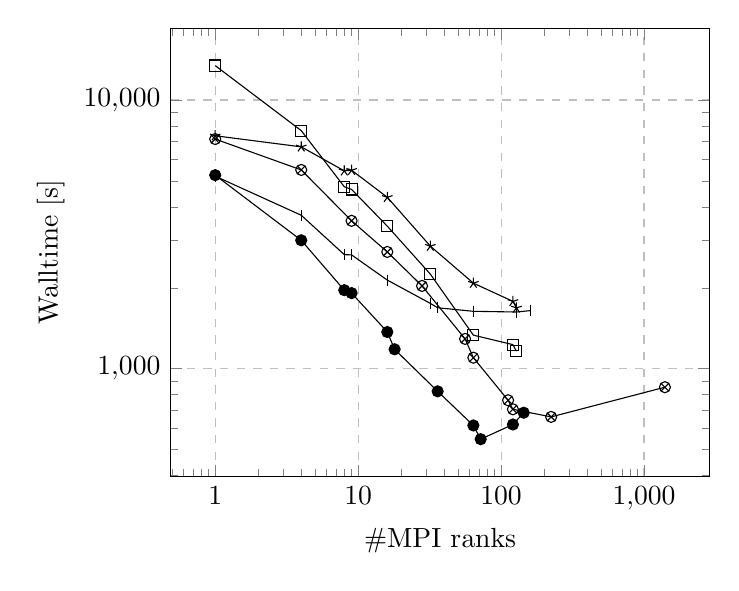
\begin{tikzpicture}[scale=1, baseline]
      \begin{axis}[
          xmode=log,
          ymode=log,
          log ticks with fixed point,
          scaled y ticks=real:1e3
          axis lines = left,
          xlabel = \#MPI ranks,
          ylabel = {Walltime [s]},
          %            legend style={at={(0.5,-0.2)},
          %            	    anchor=north,legend columns=1},
          xmajorgrids=true,
          ymajorgrids=true,
          grid style=dashed,
        ]
        %ARM
        \addplot [
          domain=1:150, 
          color=black,
          mark=square,
        ]
        coordinates {                 (1,13437.4)(4,7694.2)(8,4756.2)(9,4647.5)(16,3393.4)(32,2249)(64,1333.4)(121,1229.1)(128,1161.9)};
        %                \addlegendentry{ARM Hi1616}
        %Intel 6140
        \addplot [
          domain=1:150, 
          color=black,
          mark=*,
        ]
        coordinates {                   (1,5253.9)(4,3005.9)(8,1960.8)(9,1911.8)(16,1369.7)(18,1180.8)(36,823.6)(64,614.9)(72,546.6)(121,620.0)(144,685.8)};
        %                \addlegendentry{Intel\ Xeon\ Gold 6140}
        %AMD Epyc
        \addplot [
          domain=1:150, 
          color=black,
          mark=star,
        ]
        coordinates {
          (1,7364.1)(4,6696.0)(8,5451.3)(9,5480)(16,4345.6)(32,2859.2)(64,2081.9)(121,1781.2)(128,1683.8)};
        %               \addlegendentry{AMD Epyc 7551}
        %Eagle
        \addplot [
          domain=1:1400, 
          color=black,
          mark=otimes,
        ]
        coordinates {                    (1,7158.7)(4,5493.6)(9,3552.1)(16,2720.5)(28,2033)(56,1291.2)(64,1099.1)(112,763.1)(121,706.3)(224,661.7)(1400,853.4)
        };
        %                \addlegendentry{Eagle/Intel\ Xeon\ E5-2697 v3}
        %Power
        \addplot [
          domain=1:150, 
          color=black,
          mark=|,
        ]
        coordinates {
          (1,5208.5)(4,3725.4)(8,2658.6)(9,2652.2)(16,2137.1)(32,1750.5)(36,1686.2)(64,1635.6)(128,1625.7)(160,1644.8)
        };
        %                \addlegendentry{Power8+ S822LC}
      \end{axis}
    \end{tikzpicture}
    \caption{\textsf{Pandora}/GG scalability}
    \label{fig:pandora_scalability}
  \end{subfigure}\hfill
  \begin{subfigure}[t]{0.48\textwidth}
    \centering
    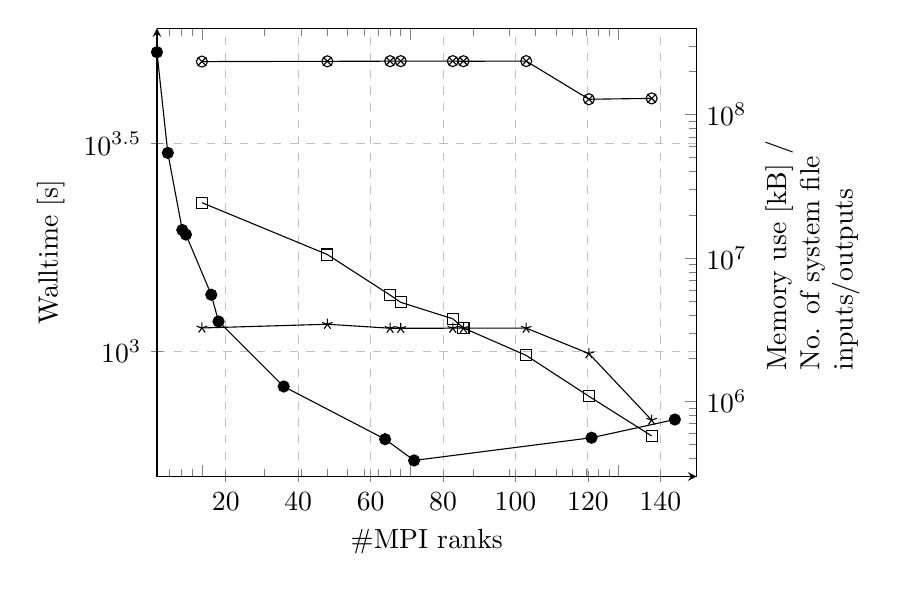
\begin{tikzpicture}[scale=1, baseline]
      \begin{axis}[
          %    width=1\textwidth,
          axis y line*=left,
          axis lines = left,
          xlabel = \#MPI ranks,
          ylabel = {Walltime [s]},
          xmajorgrids=true,
          ymajorgrids=true,
          grid style=dashed,
          xmin=1, xmax=150,
          ymode=log,
          ymin=500, ymax=6000,
        ]
        %Execution time
        \addplot [
          domain=1:70, 
          color=black,
          mark=*,
        ]
        coordinates {                   (1,5253.9)(4,3005.9)(8,1960.8)(9,1911.8)(16,1369.7)(18,1180.8)(36,823.6)(64,614.9)(72,546.6)(121,620.0)(144,685.8)};
        \label{pandora_execution_time}
      \end{axis}
      \begin{axis}[
          xmode=log,
          ymode=log,
          xticklabel=\empty,
          axis y line*=right,
          scaled ticks=false,
          y tick label style={/pgf/number format/.cd,sci,sci e},
          ymin=300000, ymax=400000000,
          ylabel style={text width=3cm},
          ylabel = {Memory use {[kB]} {/} No. of system file inputs/outputs},
          legend style={at={(0.5,-0.2)},
            anchor=north,legend columns=1},
          grid style=dashed,
        ]
        \addlegendimage{/pgfplots/refstyle=pandora_execution_time}
        %                \addlegendentry{Execution time}
        %RAM
        \addplot [
          domain=1:70, 
          color=black,
          mark=square,
        ]
        coordinates {(1,24316736)(4,10578468)(8,5519380)(9,4912336)(16,3772628)(18,3255200)(36,2096424)(72,1087508)(144,575948)};
        %               \addlegendentry{Memory use}
        %#inputs
        \addplot [
          domain=1:70, 
          color=black,
          mark=star,
        ]
        coordinates {(1,3255992)(4,3455808)(8,3243280)(9,3237968)(16,3245208)(18,3244448)(36,3249248)(72,2158432)(144,742416)};
        %               \addlegendentry{No. of system file inputs}
        %#outputs
        \addplot [
          color=black,
          mark=otimes,
        ]
        coordinates {(1,234115384)(4,235057696)(8,235684024)(9,235765544)(16,235883464)(18,235413696)(36,235913920)(72,127931040)(144,129657720)};
        %                    \addlegendentry{No. of system file outputs}
      \end{axis}
    \end{tikzpicture}
    \caption{\textsf{Pandora}/GG on Intel\ Xeon\ Gold 6140}
    \label{fig:pandora_intel_gold}
  \end{subfigure}\bigbreak
  %      \caption{Results for \textsf{Pandora}/GG (worldwide map)}
  %\end{figure}

  \caption{Results for social simulation applications}
  \label{fig:socapps_plots}
\end{figure}

%% 1 row - OpenSWPC
\begin{figure}[tphb]
  \centering
  \iffalse
  \begin{subfigure}[t]{0.48\textwidth}
    \centering
    \begin{tikzpicture}[scale=1, baseline]
      \begin{customlegend}[legend columns=1,legend style={font=\tiny, column sep=2ex},
          legend entries={Eagle/Intel\textregistered\ Xeon\textregistered\ E5-2697 v3,
            ARM Hi1616,
            Intel\textregistered\ Xeon\textregistered\ Gold 6140,
            AMD Epyc 7551,
            Power8+ S822LC
        }]
        \addlegendimage{mark=otimes,solid}
        \addlegendimage{mark=square,solid}
        \addlegendimage{mark=*,solid}
        \addlegendimage{mark=star,solid}
        \addlegendimage{mark=|,solid}
      \end{customlegend}
    \end{tikzpicture}
  \end{subfigure}\hfill
  \begin{subfigure}[t]{0.48\textwidth}
    \centering
    \begin{tikzpicture}[scale=1, baseline]
      \begin{customlegend}[legend columns=1,legend style={font=\tiny, column sep=2ex},
          legend entries={Execution time ,
            Memory use,
            No. of system file inputs,
            No. of system file outputs
        }]
        \addlegendimage{mark=*,solid}
        \addlegendimage{mark=square,solid}
        \addlegendimage{mark=star,solid}
        \addlegendimage{mark=otimes,solid}
      \end{customlegend}
    \end{tikzpicture}
  \end{subfigure}\bigbreak
  \fi
  \begin{subfigure}[t]{0.48\textwidth}
    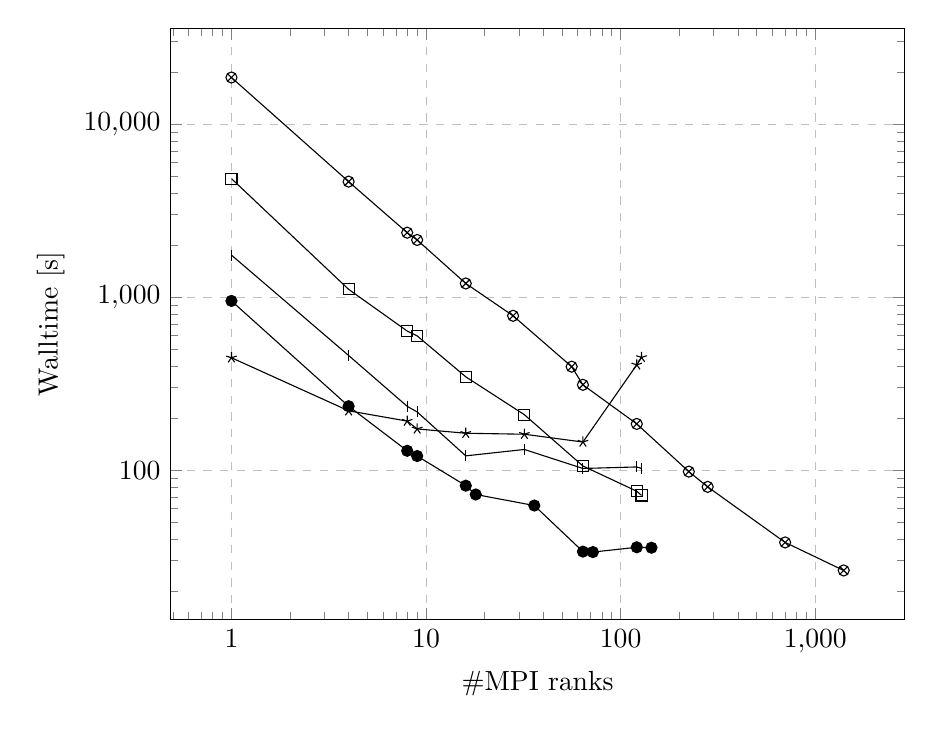
\begin{tikzpicture}[scale=1, baseline]
      \begin{axis}[width=.9\textwidth,height=.75\textwidth,
          xmode=log,
          ymode=log,
          log ticks with fixed point,
          scaled y ticks=real:1e3
          axis lines = left,
          xlabel = \#MPI ranks,
          ylabel = {Walltime [s]},
          %            legend style={at={(0.5,-0.2)},
          %            	    anchor=north,legend columns=1},
          xmajorgrids=true,
          ymajorgrids=true,
          grid style=dashed,
        ]
        %ARM
        \addplot [
          domain=1:150, 
          color=black,
          mark=square,
        ]
        coordinates {
          (1,4840)(4,1109)(8,636.4)(9,596.9)(16,346.1)(32,209.1)(64,105.6)(121,75.5)(128,71.4)
        };
        %                \addlegendentry{ARM Hi1616}
        %Intel 6140
        \addplot [
          domain=1:150, 
          color=black,
          mark=*,
        ]
        coordinates {
          (1,950.4)(4,234)(8,129.3)(9,120.6)(16,81.3)(18,72.3)(36,62.4)(64,33.8)(72,33.6)(121,35.8)(144,35.6)
        };
        %               \addlegendentry{Intel\textregistered\ Xeon\textregistered\ Gold 6140}
        %AMD Epyc
        \addplot [
          domain=1:150, 
          color=black,
          mark=star,
        ]
        coordinates {
          (1,446.1)(4,220.2)(8,192)(9,173)(16,163.3)(32,161.21)(64,145.3)(121,406)(128,448.1)
        };
        %               \addlegendentry{AMD Epyc 7551}
        %Eagle
        \addplot [
          domain=1:1400, 
          color=black,
          mark=otimes,
        ]
        coordinates {                    (1,18584.8)(4,4649.8)(8,2356.4)(9,2139.0)(16,1198.7)(28,779.8)(56,396.2)(64,311.1)(121,184.9)(224,98)(280,80)(700,38.2)(1400,26.3)
        };
        %              \addlegendentry{Eagle/Intel\textregistered\ Xeon\textregistered\ E5-2697 v3}
        %Power
        \addplot [
          domain=1:150, 
          color=black,
          mark=|,
        ]
        coordinates {
          (1,1748.7)(4,459.8)(8,233.7)(9,216.9)(16,120.9)(32,131.6)(64,102.2)(121,104.3)(128,102.2)
        };
        %                \addlegendentry{Power8+ S822LC}
      \end{axis}
    \end{tikzpicture}
    \caption{OpenSWPC scalability}
    \label{fig:openswpc_scalability}
  \end{subfigure}\hfill
  \begin{subfigure}[t]{0.48\textwidth}
    \centering
    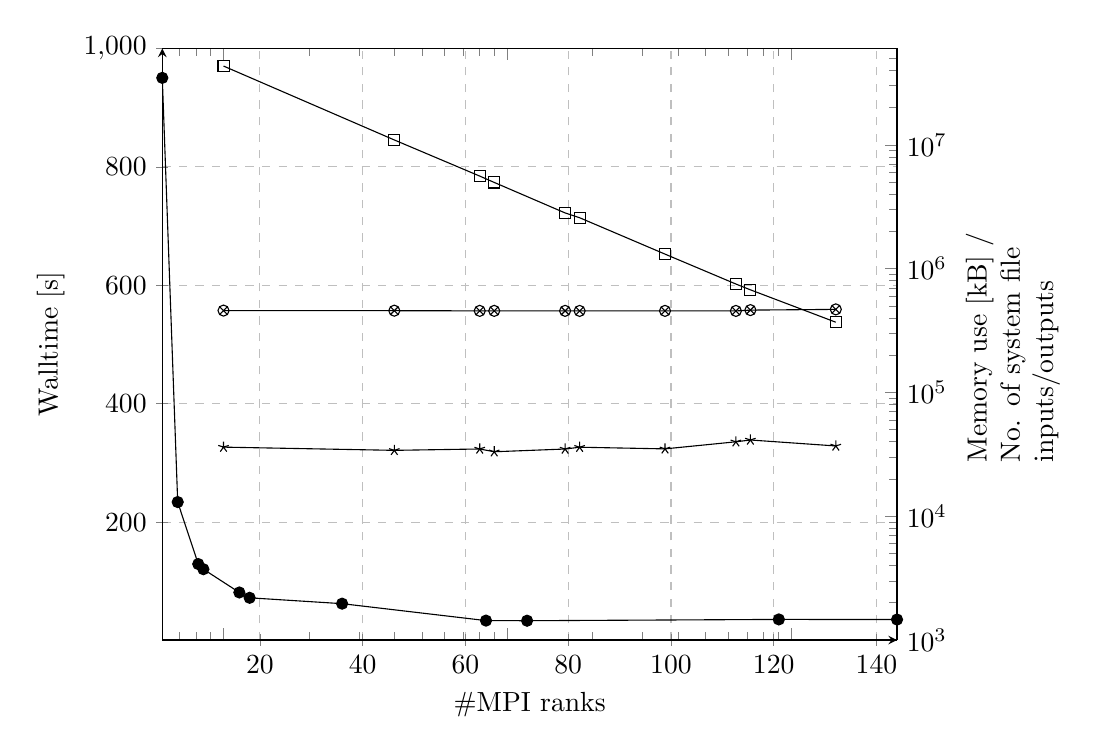
\begin{tikzpicture}[scale=1, baseline]
      \begin{axis}[width=.9\textwidth,height=.75\textwidth,
          %    width=1\textwidth,
          axis y line*=left,
          axis lines = left,
          xlabel = \#MPI ranks,
          ylabel = {Walltime [s]},
          xmajorgrids=true,
          ymajorgrids=true,
          grid style=dashed,
          ymin=1, ymax=1000,
        ]
        %Execution time
        \addplot [
          domain=1:70, 
          color=black,
          mark=*,
        ]
        coordinates {(1,950.4)(4,234)(8,129.3)(9,120.6)(16,81.3)(18,72.3)(36,62.4)(64,33.8)(72,33.6)(121,35.8)(144,35.6)};
        \label{openswpc_execution_time}
      \end{axis}
      \begin{axis}[width=.9\textwidth,height=.75\textwidth,
          xmode=log,
          ymode=log,
          xticklabel=\empty,
          axis y line*=right,
          scaled ticks=false,
          y tick label style={/pgf/number format/.cd,sci,sci e},
          ymin=1000, ymax=60000000,
          ylabel style={text width=3cm},
          ylabel = {Memory use {[kB]} {/} No. of system file inputs/outputs},
          legend style={at={(0.5,-0.2)},
            anchor=north,legend columns=1},
          grid style=dashed,
        ]
        \addlegendimage{/pgfplots/refstyle=openswpc_execution_time}
        %                \addlegendentry{Execution time}
        %RAM
        \addplot [
          domain=1:70, 
          color=black,
          mark=square,
        ]
        coordinates {(1,43267296)(4,10943064)(8,5590132)(9,4967892)(16,2816788)(18,2576328)(36,1309532)(64,751016)(72,674056)(144,368968)};
        %                \addlegendentry{Memory use}
        %#inputs
        \addplot [
          domain=1:70, 
          color=black,
          mark=star,
        ]
        coordinates {(1,36144)(4,34048)(8,34920)(9,33160)(16,34896)(18,36088)(36,34992)(64,39920)(72,41272)(144,36944)};
        %               \addlegendentry{No. of system file inputs}
        %#outputs
        \addplot [
          color=black,
          mark=otimes,
        ]
        coordinates {(1,458040)(4,457256)(8,455752)(9,455664)(16,455688)(18,455248)(36,455544)(64,455168)(72,462144)(144,468512)};
        %                    \addlegendentry{No. of system file outputs}
      \end{axis}
    \end{tikzpicture}
    \caption{OpenSWPC on Intel Xeon Gold 6140}
    \label{fig:openswpc_intel_gold}
  \end{subfigure}\bigbreak
  %      \caption{Results for OpenSWPC}
  %\end{figure}


  %%2 row - CMAQ/CCTM
  %\begin{figure}[ht]
  %\centering
  \begin{subfigure}[t]{0.48\textwidth}
    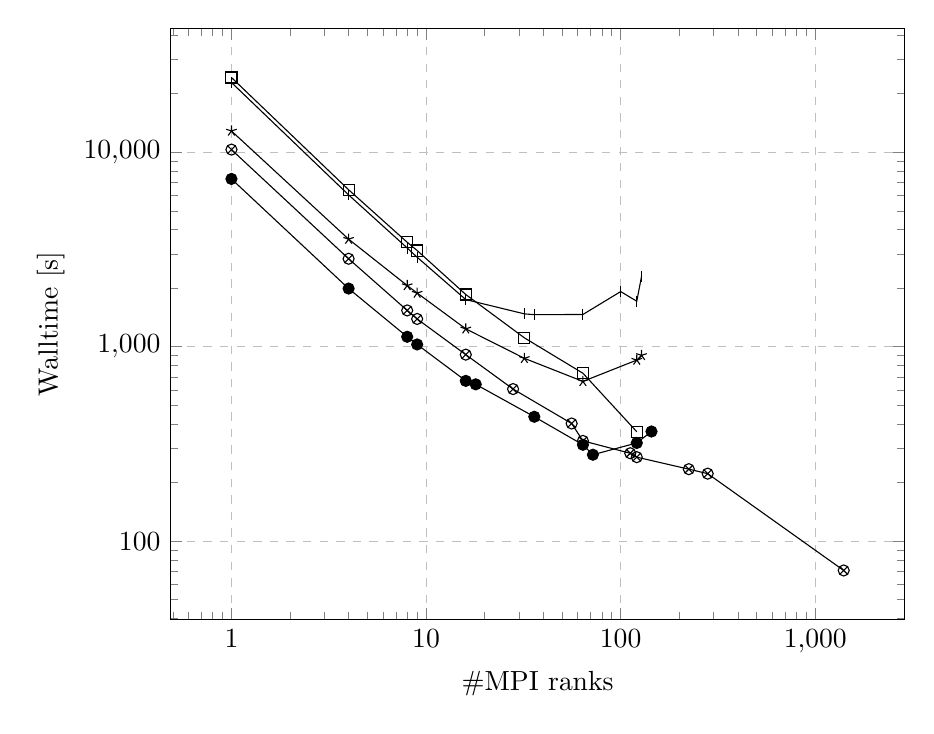
\begin{tikzpicture}[scale=1, baseline]
      \begin{axis}[width=.9\textwidth,height=.75\textwidth,
          %    width=1.3\textwidth,
          xmode=log,
          ymode=log,
          log ticks with fixed point,
          scaled y ticks=real:1e3
          axis lines = left,
          xlabel = \#MPI ranks,
          ylabel = {Walltime [s]},
          %        legend style={at={(0.5,-0.2)},
          %        	    anchor=north,legend columns=1},
          xmajorgrids=true,
          ymajorgrids=true,
          grid style=dashed,
        ]
        %ARM
        \addplot [
          domain=1:150, 
          color=black,
          mark=square,
        ]
        coordinates {
          (1,24239.6)(4,6416.1)(8,3445.6)(9,3124.6)(16,1856.3)(32,1111.4)(64,730.7)(121,365.4)
        };
        %        \addlegendentry{ARM Hi1616}
        %Intel 6140
        \addplot [
          domain=1:150, 
          color=black,
          mark=*,
        ]
        coordinates {
          (1,7294.6)(4,1991.6)(8,1125.1)(9,1027.3)(16,667.5)(18,640.7)(36,436.4)(64,313.2)(72,278.4)(121,320)(144,366.5)
        };
        %        \addlegendentry{Intel\textregistered\ Xeon\textregistered\ Gold 6140}
        %AMD Epyc
        \addplot [
          domain=1:150, 
          color=black,
          mark=star,
        ]
        coordinates {
          (1,12872.6)(4,3574.8)(8,2064.3)(9,1888.6)(16,1235.9)(32,871.8)(64,663.3)(121,853.9)(128,902.9)
        };
        %        \addlegendentry{AMD Epyc 7551}
        %Eagle
        \addplot [
          domain=1:1400,
          color=black,
          mark=otimes,
        ]
        coordinates {
          (1,10323.7)(4,2834.3)(8,1537)(9,1389.7)(16,910.7)(28,605.8)(56,402.9)(64,327.9)(112,283.3)(121,270.5)(224,234.6)(280,222.5)(1400,70.7)
        };
        %       \addlegendentry{Eagle/Intel\textregistered\ Xeon\textregistered\ E5-2697 v3}
        %Power
        \addplot [
          domain=1:150, 
          color=black,
          mark=|,
        ]
        coordinates {
          (1,22849.8)(4,6036.1)(8,3220.3)(9,2885.9)(16,1748.2)(32,1476)(36,1461.4)(64,1465.4)(100,1921.8)(121,1714.5)(128,2297.7)
        };
        %      \addlegendentry{Power8+ S822LC}
      \end{axis}
    \end{tikzpicture}
    \caption{CMAQ/CCTM scalability}
    \label{fig:cmaq_scalability}
  \end{subfigure}\hfill
  \begin{subfigure}[t]{0.48\textwidth}
    \centering
    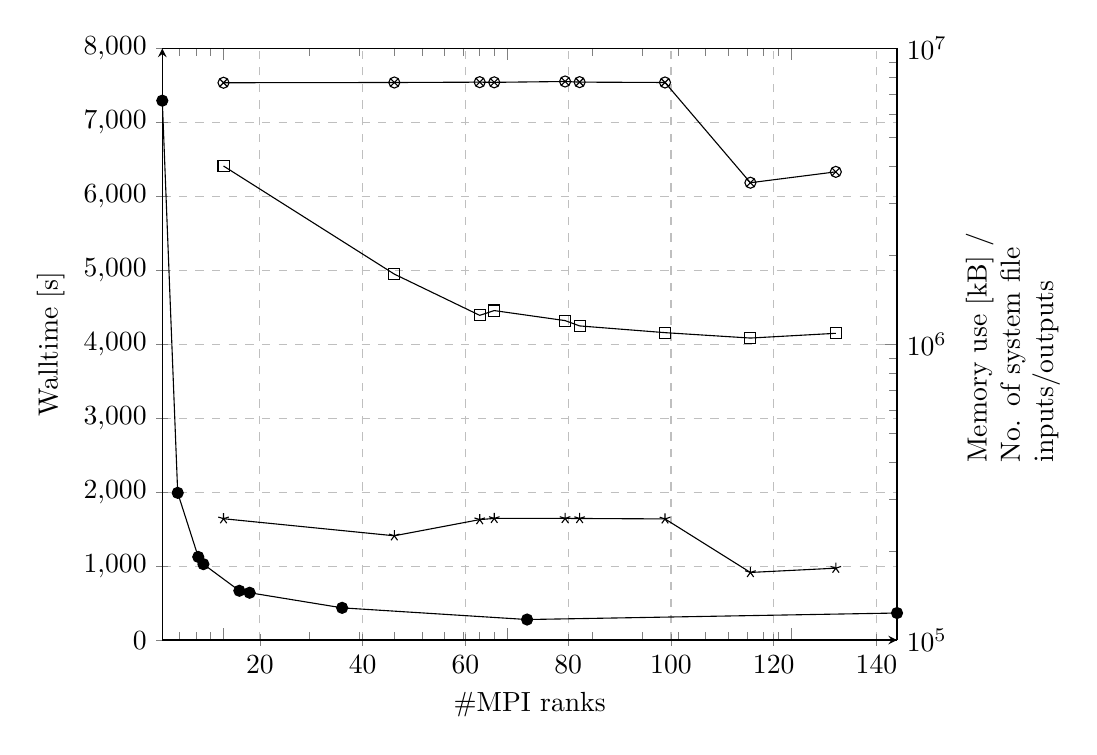
\begin{tikzpicture}[scale=1, baseline]
      \begin{axis}[width=.9\textwidth,height=.75\textwidth,
          %    width=1\textwidth,
          axis y line*=left,
          axis lines = left,
          xlabel = \#MPI ranks,
          ylabel = {Walltime [s]},
          xmajorgrids=true,
          ymajorgrids=true,
          grid style=dashed,
          ymin=1, ymax=8000,
        ]
        %Execution time
        \addplot [
          domain=1:70, 
          color=black,
          mark=*,
        ]
        coordinates {(1,7294.6)(4,1991.4)(8,1125.1)(9,1027.3)(16,667.5)(18,640.7)(36,436.4)(72,278.4)(144,366.5)};
        \label{cmaq_execution_time}
      \end{axis}
      \begin{axis}[width=.9\textwidth,height=.75\textwidth,
          xmode=log,
          ymode=log,
          xticklabel=\empty,
          axis y line*=right,
          scaled ticks=false,
          y tick label style={/pgf/number format/.cd,sci,sci e},
          ymin=100000, ymax=10000000,
          ylabel style={text width=3cm},
          ylabel = {Memory use {[kB]} {/} No. of system file inputs/outputs},
          %                legend style={at={(0.5,-0.2)},
          %                	    anchor=north,legend columns=1},
          grid style=dashed,
        ]
        \addlegendimage{/pgfplots/refstyle=cmaq_execution_time}
        %                \addlegendentry{Execution time}
        %RAM
        \addplot [
          domain=1:70, 
          color=black,
          mark=square,
        ]
        coordinates {(1,4005556)(4,1726776)(8,1252488)(9,1299756)(16,1202224)(18,1153424)(36,1094592)(72,1049436)(144,1089048)};
        %                \addlegendentry{Memory use}
        %#inputs
        \addplot [
          domain=1:70, 
          color=black,
          mark=star,
        ]
        coordinates {(1,257120)(4,225160)(8,255344)(9,257736)(16,257736)(18,257592)(36,256752)(72,169256)(144,174968)};
        %               \addlegendentry{No. of system file inputs}
        %#outputs
        \addplot [
          color=black,
          mark=otimes,
        ]
        coordinates {(1,7660576)(4,7674568)(8,7695080)(9,7684712)(16,7735376)(18,7696800)(36,7676016)(72,3516968)(144,3827848)};
        %                \addlegendentry{No. of system file outputs}
      \end{axis}
    \end{tikzpicture}
    %          \caption{CMAQ/CCTM detailed results for Intel\textregistered\ Xeon\textregistered\ Gold 6140}
    \caption{CMAQ/CCTM on Intel Xeon Gold 6140}
    \label{fig:cmaq_intel_gold}
  \end{subfigure}\bigbreak
  %    \caption{Results for CMAQ/CCTM}


  %%3 row - CM1

  \begin{subfigure}[t]{0.48\textwidth}
    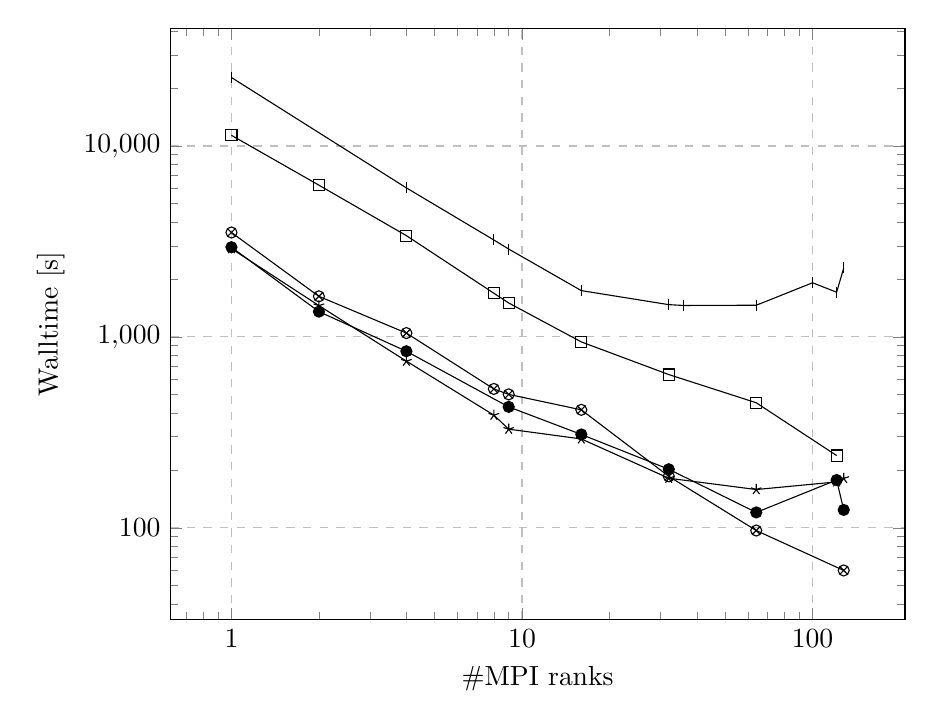
\begin{tikzpicture}[scale=1, baseline]
      \begin{axis}[width=.9\textwidth,height=.75\textwidth,
          xmode=log,
          ymode=log,
          log ticks with fixed point,
          scaled y ticks=real:1e3
          axis lines = left,
          xlabel = \#MPI ranks,
          ylabel = {Walltime [s]},
          %            legend style={at={(0.5,-0.2)},
          %            	    anchor=north,legend columns=1},
          xmajorgrids=true,
          ymajorgrids=true,
          grid style=dashed,
        ]
        %ARM
        \addplot [
          domain=1:150, 
          color=black,
          mark=square,
        ]
        coordinates {
          (1,11379.8)(2,6236)(4,3393.1)(8,1694.1)(9,1505.9)(16,941.5)(32,635.1)(64,452)(121,239.1)
        };
        %           \addlegendentry{ARM Hi1616}
        %Intel 6140
        \addplot [
          domain=1:150, 
          color=black,
          mark=*,
        ]
        coordinates {
          (1,2952)(2,1356.7)(4,841.2)(9,430)(16,308.4)(32,202.7)(64,120.4)(121,178)(128,124.1)
        };
        %          \addlegendentry{Intel\textregistered\ Xeon\textregistered\ Gold 6140}
        %AMD Epyc
        \addplot [
          domain=1:150, 
          color=black,
          mark=star,
        ]
        coordinates {
          (1,2900)(2,1459)(4,746.8)(8,389.4)(9,328.7)(16,292.2)(32,181.9)(64,158.7)(121,174)(128,181.5)
        };
        %            \addlegendentry{AMD Epyc 7551}
        %Eagle
        \addplot [
          domain=1:1400,
          color=black,
          mark=otimes,
        ]
        coordinates {
          (1,3524)(2,1631.4)(4,1047.2)(8,534)(9,500)(16,415)(32,186.1)(64,96.8)(128,59.8)
        };
        %           \addlegendentry{Eagle/Intel\textregistered\ Xeon\textregistered\ E5-2697 v3}
        %Power
        \addplot [
          domain=1:150, 
          color=black,
          mark=|,
        ]
        coordinates {
          (1,22849.8)(4,6036.1)(8,3220.3)(9,2885.9)(16,1748.2)(32,1476)(36,1461.4)(64,1465.4)(100,1921.8)(121,1714.5)(128,2297.7)
        };
        %          \addlegendentry{Power8+ S822LC}
      \end{axis}
    \end{tikzpicture}
    \caption{CM1\ scalability}
    \label{fig:cm1_scalability}
  \end{subfigure}\hfill
  \begin{subfigure}[t]{0.48\textwidth}
    \centering
    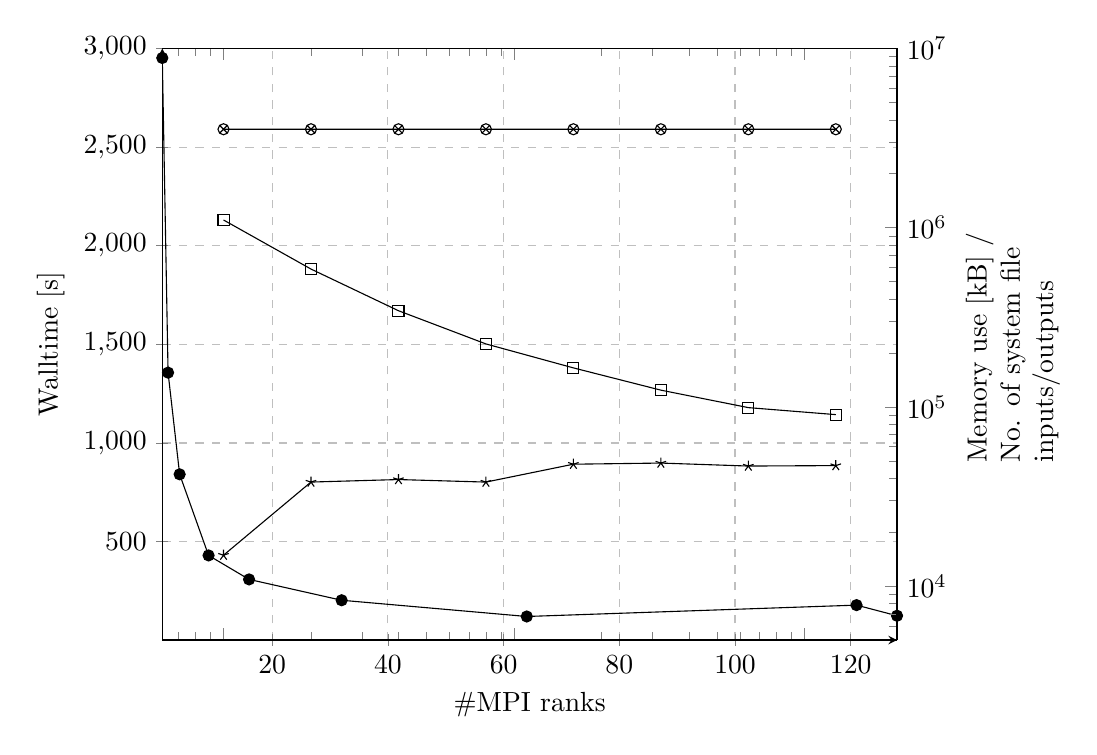
\begin{tikzpicture}[scale=1, baseline]
      \begin{axis}[width=.9\textwidth,height=.75\textwidth,
          %    width=1\textwidth,
          axis y line*=left,
          axis lines = left,
          xlabel = \#MPI ranks,
          ylabel = {Walltime [s]},
          xmajorgrids=true,
          ymajorgrids=true,
          grid style=dashed,
          ymin=1, ymax=3000,
        ]
        %Execution time
        \addplot [
          domain=1:70, 
          color=black,
          mark=*,
        ]
        coordinates {
          (1,2952)(2,1356.7)(4,841.2)(9,430)(16,308.4)(32,202.7)(64,120.4)(121,178)(128,124.1)};
        \label{cm1_execution_time}
      \end{axis}
      \begin{axis}[width=.9\textwidth,height=.75\textwidth,
          xmode=log,
          ymode=log,
          xticklabel=\empty,
          axis y line*=right,
          scaled ticks=false,
          y tick label style={/pgf/number format/.cd,sci,sci e},
          ymin=5000, ymax=10000000,
          ylabel style={text width=3cm},
          ylabel = {Memory use {[kB]} {/} No. of system file inputs/outputs
          },
          legend style={at={(0.5,-0.2)},
            anchor=north,legend columns=1},
          grid style=dashed,
        ]
        \addlegendimage{/pgfplots/refstyle=cm1_execution_time}
        %            \addlegendentry{Execution time}
        %RAM
        \addplot [
          domain=1:70, 
          color=black,
          mark=square,
        ]
        coordinates {(1,1104060)(2,587776)(4,344076)(8,224576)(16,165060)(32,124016)(64,99052)(128,90536)};
        %            \addlegendentry{Memory use}
        %#inputs
        \addplot [
          domain=1:70, 
          color=black,
          mark=star,
        ]
        coordinates {(1,14872)(2,38064)(4,39312)(8,38056)(16,47880)(32,48584)(64,46760)(128,47032)};
        %           \addlegendentry{No. of system file inputs}
        %#outputs
        \addplot [
          color=black,
          mark=otimes,
        ]
        coordinates {(1,3542800)(2,3542536)(4,3542224)(8,3541976)(16,3541912)(32,3541784)(64,3541336)(128,3541336)};
        %            \addlegendentry{No. of system file outputs}
      \end{axis}
    \end{tikzpicture}
    %  \caption{CM1 detailed results for Intel\textregistered\ Xeon\textregistered\ Gold 6140}
    \caption{CM1 on Intel Xeon Gold 6140}
    \label{fig:cm1_intel_gold}
  \end{subfigure}%
  %  \caption{Results for CM1}
  %\end{figure}

  %%4 row - HWRF
  %\begin{figure}[ht]
  \begin{subfigure}[t]{0.48\textwidth}
    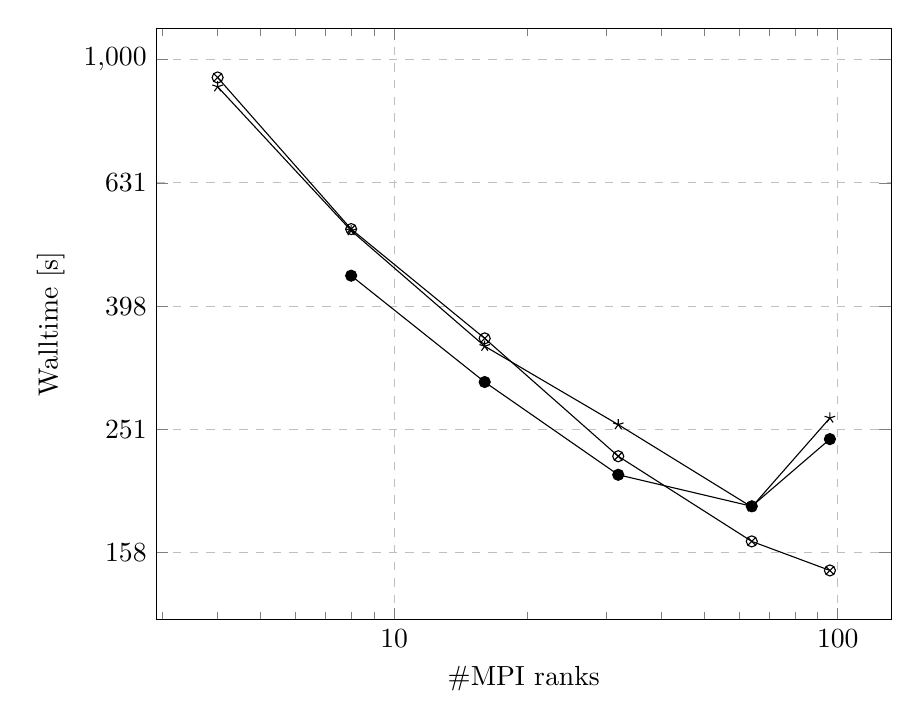
\begin{tikzpicture}[scale=1, baseline]
      \begin{axis}[width=.9\textwidth,height=.75\textwidth,
          xmode=log,
          ymode=log,
          log ticks with fixed point,
          scaled y ticks=real:1e3
          axis lines = left,
          xlabel = \#MPI ranks,
          ylabel = {Walltime [s]},
          %           legend style={at={(0.5,-0.2)},
          %            	    anchor=north,legend columns=1},
          xmajorgrids=true,
          ymajorgrids=true,
          grid style=dashed,
        ]
        %Intel 6140
        \addplot [
          domain=1:150, 
          color=black,
          mark=*,
        ]
        coordinates {(8,446)(16,299.8)(32,212)(64,188.5)(96,242.2)};
        %           \addlegendentry{Intel\textregistered\ Xeon\textregistered\ Gold 6140}
        %AMD Epyc
        \addplot [
          domain=1:150, 
          color=black,
          mark=star,
        ]
        coordinates {
          (4,903.4)(8,527.7)(16,342.7)(32,255.7)(64,188)(96,262.1)
        };
        %          \addlegendentry{AMD Epyc 7551}
        %Eagle
        \addplot [
          domain=1:1400,
          color=black,
          mark=otimes,
        ]
        coordinates {
          (4,935)(8,530.8)(16,352.9)(32,227.2)(64,165.3)(96,148.3)                };
        %          \addlegendentry{Eagle/Intel\textregistered\ Xeon\textregistered\ E5-2697 v3}
      \end{axis}
    \end{tikzpicture}
    \caption{HWRF\ scalability}
    \label{fig:hwrf_scalability}
  \end{subfigure}\hfill
  \begin{subfigure}[t]{0.48\textwidth}
    \centering
    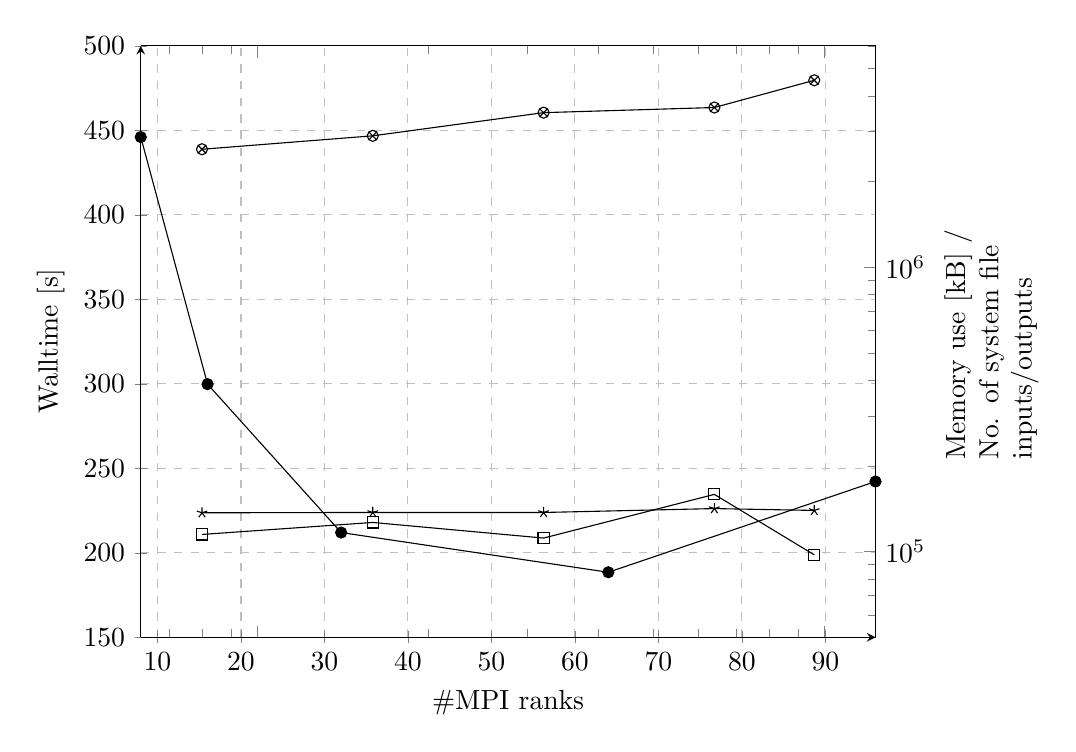
\begin{tikzpicture}[scale=1, baseline]
      \begin{axis}[width=.9\textwidth,height=.75\textwidth,
          axis y line*=left,
          axis lines = left,
          xlabel = \#MPI ranks,
          ylabel = {Walltime [s]},
          xmajorgrids=true,
          ymajorgrids=true,
          grid style=dashed,
          ymin=150, ymax=500,
        ]
        %Execution time
        \addplot [
          domain=1:70, 
          color=black,
          mark=*,
        ]
        coordinates {(8,446)(16,299.8)(32,212)(64,188.5)(96,242.2)};
        \label{hwrf_execution_time}
      \end{axis}
      \begin{axis}[width=.9\textwidth,height=.75\textwidth,
          xmode=log,
          ymode=log,
          xticklabel=\empty,
          axis y line*=right,
          scaled ticks=false,
          y tick label style={/pgf/number format/.cd,sci,sci e},
          ymin=50000, ymax=6000000,
          ylabel style={text width=3cm},
          ylabel = {Memory use {[kB]} {/} No. of system file inputs/outputs
          },
          %            legend style={at={(0.5,-0.2)},
          %            	    anchor=north,legend columns=1},
          grid style=dashed,
        ]
        \addlegendimage{/pgfplots/refstyle=hwrf_execution_time}
        %            \addlegendentry{Execution time}
        %RAM
        \addplot [
          domain=1:70, 
          color=black,
          mark=square,
        ]
        coordinates {(8,114972)(16,126672)(32,111652)(64,158992)(96,97456)};
        %           \addlegendentry{Memory use}
        %#inputs
        \addplot [
          domain=1:70, 
          color=black,
          mark=star,
        ]
        coordinates {(8,136992)(16,137352)(32,137332)(64,141736)(96,139632)};
        %          \addlegendentry{No. of system file inputs}
        %#outputs
        \addplot [
          color=black,
          mark=otimes,
        ]
        coordinates {(8,2596976)(16,2895408)(32,3492632)(64,3641504)(96,4538256)};
        %          \addlegendentry{No. of system file outputs}
      \end{axis}
    \end{tikzpicture}
    \caption{HWRF on Intel\textregistered\ Xeon\textregistered\ Gold 6140}
    \label{fig:hwrf_gold}
  \end{subfigure}\bigbreak
  \caption{Results for CFD applications}
  \label{fig:cfdapps_plots}
\end{figure}



The group of benchmarked social simulation software covers applications for pre-processing and simulation of agent-based models.
In order to study computational requirements to applications that generate synthetic populations,
a simple parallel version of the celebrated iterative proportional fitting (IPF) method was implemented.
This implementation heavily uses dense linear algebra kernels provided by a highly optimised ScaLAPACK library.
The benchmarks demonstrate high performance of IPF on different architectures.
Neither RAM, nor I/O of modern architectures are limiting factors for IPF performance.
Along with ABMS pre-processing applications,
a simple agent-based model of diffusion with the help of distributed ABMS frameworks
following two different parallelization strategies for ABMs with raster inputs was benchmarked.
The first framework (Pandora) written in C++ parallelises
the simulation process via splitting of rasters on even pieces and distributing them between MPI processes,
while the second framework (ABM4py) is a Python code,
which implements the graph-based parallelization approach.
Despite strong difference in parallelization strategies, in both cases, the observation delivered the same pattern:
ABMS applications produce a big amount of output which has a strong negative impact on application performance.
As a consequence, according to the "toy" ABMs, being I/O bound, current ABMS frameworks for HPC have moderate requirements to CPU performance. Nevertheless, it must be emphasised that the results can look differently for complex models with sophisticated agent activities and models which can be reduced to iterations with sparse-matrix dense-vector operations, thus, the benchmarks for ABMS frameworks are not very illuminative and must be extended with more sophisticated models to draw stronger conclusions. But discussion of the new ABMS models for benchmarking goes beyond the scope of this text. Table~\ref{tab:bottlenecks_hardware} shortly summarises information about scalability of the benchmarked social simulation software and hardware bottlenecks.

\begin{table}[htbp]
\begin{minipage}{1\textwidth}
\caption{Bottlenecks in the hardware and scalability for the application from social simulation software stack}
\label{tab:bottlenecks_hardware}
\end{minipage}
\begin{tabular}{cl|c|c|c|c|}
\cline{3-6}
 &  & {pre-processing} & \multicolumn{3}{c|}{ABMS (with raster input)} \\ \cline{3-6} 
 &  & \multirow{2}{*}{IPF} & \multicolumn{2}{c|}{Pandora} & \multicolumn{1}{l|}{ABM4py} \\ \cline{4-6} 
 &  &  & \multicolumn{1}{l|}{Europe} & \multicolumn{1}{l|}{World} & \multicolumn{1}{l|}{128x128} \\ \hline
\multicolumn{1}{|c|}{\multirow{4}{*}{Bottlenecks}} & CPU & \checkmark &  &  &  \\ \cline{2-6} 
\multicolumn{1}{|c|}{} & RAM &  &  &  &  \\ \cline{2-6} 
\multicolumn{1}{|c|}{} & IO  &  & output & output & output \\ \cline{2-6} 
\multicolumn{1}{|c|}{} & Network&  &  &  &  \\ \hline
\multicolumn{2}{|c|}{Scalability \ *} & $\ge$1400 &  $\approx$128 & $\approx$700 & $\approx$128 \\ \hline
\end{tabular}
\newline
\raggedright{* maximum\ number\ of\ utilised\ cores\ for\ Eagle\ cluster}
\end{table}




The group of benchmarked CFD applications includes large scale tools that simulate GSS-related scenarios like natural disasters (hurricanes, earthquakes), spread of air pollution and weather prediction. More specifically, the following open-source CFD codes have been selected the benchmarking purposes: HRWF – a parallel implementation of the hurricane weather research and forecasting (HWRF); OpenSWPC – an integrated parallel simulation code for modelling seismic wave propagation in 3D heterogeneous viscoelastic media; CMAQ – a community multiscale air quality modelling system, which combines CFD codes for conducting large scale air quality model simulations.

As expected, the benchmarks confirm that CFD applications are in general CPU-bound (e.g. Figure~\ref{fig:openswpc_scalability}) in contrast to the social simulation software. At the same, time output makes a solid contribution to the total elapsed time for such applications like CCTM and CM1 (e.g. Figure~\ref{fig:cm1_intel_gold}) which, in turn, imposed additional performance constraints on architectures with poor I/O speed. Nevertheless, it was observed that at some architectures memory was also a bottleneck for some choices of the number of MPI processes. In addition, it was noticed that OpenSWPC is memory bound for the small number of MPI processes. The relevant information about scalability of the benchmarked CFD applications and hardware bottlenecks is outlined it Table~\ref{tab:bottlenecks_cfd_hardware}.


\begin{table}[hbtp]
\begin{minipage}{1\textwidth}
\caption{Bottlenecks in the hardware and scalability for the large-scale CFD applications}
\label{tab:bottlenecks_cfd_hardware}
\end{minipage}
\begin{tabular}{cl|c|c|c|c|}
\cline{3-6}
 &  & HWRF & OpenSWPC & CMAQ/CCTM) & \multicolumn{1}{l|}{CM1} \\ \hline
\multicolumn{1}{|c|}{\multirow{4}{*}{Bottlenecks}} & CPU & \checkmark & \checkmark & \checkmark & \checkmark \\ \cline{2-6} 
\multicolumn{1}{|c|}{} & RAM &  & \checkmark &  &  \\ \cline{2-6} 
\multicolumn{1}{|c|}{} & IO & input &  & output & output \\ \cline{2-6} 
\multicolumn{1}{|c|}{} & Network &  &  &  &  \\ \hline
\multicolumn{2}{|c|}{Scalability *} & $\ge$128 & $\ge$128 & $\ge$128 & $\ge$128 \\ \hline
\end{tabular}
\newline
\raggedright{* maximum\ number\ of\ utilised\ cores\ for\ Eagle\ cluster}
\end{table}






As Tables ~\ref{tab:bottlenecks_hardware} and~\ref{tab:bottlenecks_cfd_hardware} illustrate, most of the distributed GSS applications are memory bound. Even large-scale CFD codes can be bound by I/O and RAM under special circumstances. It allows to formulate the conclusion that the fast memory is an essential requirement to HPC clusters for GSS applications whereas high CPU’s clock frequency plays a less important role. Moreover, since many state-of-the-art GSS applications deal with large input and output files, it is believed that GSS software developers should invest more time into designing file-avoiding applications. The scalability tests show that hyperthreading provides little performance improvements for most of the GSS applications. Therefore, it makes little sense to invest money in expensive massively multithreaded chips (like Power8) for GSS users. It is also recommended to avoid clusters with GPU accelerated nodes since only few popular GSS applications benefit from GPUs. In particular, among widely used general-purpose ABMS frameworks and problem-specific ABMS codes for HPCs, only the FLAME-GPU (Flexible Larg-scale Agent Modelling Environment) \cite{2011:flame_gpu} \cite{2018:flame_gpu} framework utilises GPUs. Weak use of GPUs is also partially related to the fact that most social science applications are memory bound. Being more specific, among the architectures used in benchmarking, we recommend to build clusters upon ARM Hi1616 if energy efficiency is a crucial requirement, or upon Intel\textregistered\ Xeon\textregistered\ Gold 6140 if performance is a first priority while relatively high operating expense and capital expenditure are not an issue.


